\documentclass[conference]{IEEEtran}
%Template version as of 6/27/2024

\usepackage[T1]{fontenc}
\usepackage{cite}
\usepackage{url}
\usepackage{amsmath,amssymb,amsfonts}
\usepackage{algorithmic}
\usepackage{graphicx}
\graphicspath{{./images/}}
\usepackage{textcomp}
\usepackage{xcolor}
% \usepackage[UTF8]{ctex}
% \usepackage[english]{babel}
\usepackage{microtype}
\usepackage{multirow}
\usepackage{booktabs}   
\usepackage{adjustbox}
\def\BibTeX{{\rm B\kern-.05em{\sc i\kern-.025em b}\kern-.08em
    T\kern-.1667em\lower.7ex\hbox{E}\kern-.125emX}}

\newcommand{\todo}[1]{\textcolor{red}{TODO: #1}}
\begin{document}

\title{DualAttWaveNet: Multiscale Attention Networks for Satellite Interference Detection}

\author{
    \IEEEauthorblockN{
        Chunyu Yang\IEEEauthorrefmark{1},
        Boyu Yang\IEEEauthorrefmark{2},
        Kun Qiu\IEEEauthorrefmark{3},
        Yue Gao\IEEEauthorrefmark{4}
    }
    \IEEEauthorblockA{
        School of Computer Science, Fudan University, China\\
        \IEEEauthorrefmark{1} 22307140114@m.fudan.edu.cn, 
        \IEEEauthorrefmark{2} 24110240144@m.fudan.edu.cn, \\
        \IEEEauthorrefmark{3} qkun@fudan.edu.cn, 
        \IEEEauthorrefmark{4} gao.yue@fudan.edu.cn
    }
}




\maketitle

\begin{abstract}
    The increasing number of non-geostationary orbit satellites (NGSOs) and their frequency bands overlap with geostationary orbit satellites (GSOs) have made interference detection very important. A good interference detection method can help adapt to dynamic environments and check simulation results after satellite launches. Previous works use deep learning anomaly detection that involves training an encoder-decoder model and compare input-output differences with thresholds to ensure robustness. The state-of-the-art model, TrID (transformer-based interference detector), applies transformer encoder to process input feature maps, achieving best AUC 0.8318 and F1-score 0.8321. But its multi-head attention has high computational cost. Also, TrID trains two models separately for time-domain and frequency-domain inputs, ignoring their connections. To overcome these problems, we propose DualAttWaveNet. It takes both time and frequency signals as input, fuses them by a novel bidirectional attention method, and employs wavelet regularization loss. We train the model on public dataset which consists of 28 hour of satellite signals. Experiments show compared to TrID, DualAttWaveNet improves AUC by 12\% and reduces inference time by 50\% while maintaining F1-score. \end{abstract}

\begin{IEEEkeywords}
    interference detection, multimodal fusion, bidirectional attention, wavelet transform
\end{IEEEkeywords}

\section{Introduction}
\label{sec:intro}

The accelerated deployment of low Earth orbit (LEO) satellite systems poses huge challenges for next-generation communication networks, with over 20,000 satellites projected to be launched by leading operators including SpaceX's Starlink\cite{starlink} and Starshield \cite{spacex_starshield}, as well as Eutelsat OneWeb \cite{oneweb}. These mega-constellations have become critical infrastructure to enable global connectivity, driving the commercialization of space-based communications while expanding broadband access to underserved regions \cite{reddyLowEarthOrbit2023}. However, the exponential growth in satellite numbers brings fundamental technical obstacles. Rising risk of spectrum overlap between LEO and geosynchronous orbit (GSO) satellites creates urgent demands for scalable interference management frameworks that can evolve with expanding LEO networks.

Current research in satellite interference management primarily centers on three domains: preventive measures targeting pre-deployment risk minimization \cite{sharmaInlineInterferenceMitigation2016, liOptimalBeamPower2019}, static mitigation protocols \cite{wangCoFrequencyInterferenceAnalysis2020, zhangSpectralCoexistenceLEO2018}, and simulation-driven prediction models optimized through discrete time or spatial sampling \cite{wangCoFrequencyInterferenceAnalysis2020}. While these approaches have advanced interference governance under controlled assumptions, they face critical limitations when confronting the unpredictable dynamics of space environments. The satellite networks must contend with time varying disturbances, including fluctuations in solar radiation and variations in atmospheric conditions, among other factors \cite{facskoSpaceWeatherEffects2023}. Furthermore, reliance on conventional detection methods, often dependent on fixed thresholds or static signal characteristics, struggles to address the escalating complexity of real-time interference identification. These challenges demonstrate an urgent need for effective detection mechanisms capable of rapid response to interference patterns and seamless integration with evolving physical-layer dynamics, without compromising the accuracy requirements of simulation-based validation.

Current approaches to interference detection in satellite communications can be broadly categorized into traditional analytical methods and machine learning (ML)-based methods. Conventional techniques typically use  energy detection (ED), which quantifies signal energy over fixed intervals for threshold-based anomaly identification \cite{kay2009fundamentals}. Others exploit spectral features, including cyclostationary analysis, to differentiate interference from periodic communication signals \cite{experimentalCyclostationary}. In contrast, ML-driven methods address detection through two paradigmatic lenses: classification and signal reconstruction. Classification-based approaches utilize deep neural networks to analyze in-phase/quadrature (IQ) samples or temporal signal representations, assigning interference labels via learned decision boundaries \cite{pellacoSpectrumPredictionInterference2019}. Conversely, encoder-decoder architectures formulate detection as an anomaly discrimination task by training models to reconstruct idealized interference-free waveforms from raw inputs, with deviations between original and reconstructed signals indicating potential interference \cite{saifaldawlaConvolutionalAutoencodersNonGeostationary2024}. Recent innovations further integrate transformer mechanisms to capture long-range spectral dependencies, enhancing sensitivity to long-horizen anomalies \cite{saifaldawlaGenAIBasedModelsNGSO2024}.

Despite advancements, critical challenges persist in existing interference detection methods. First, threshold-dependent traditional methods — exemplified by energy detection — exhibit degraded reliability in low-SNR regimes, where static thresholds fail to dynamically adapt to noise fluctuations or interference intensity variations, leading to frequent false negatives in rapidly evolving orbital conditions \cite{saifaldawlaGenAIBasedModelsNGSO2024}. Second, while attention-driven architectures achieve state-of-the-art detection sensitivity, their computational overhead from multi-head attention mechanisms imposes huge latency during both training and inference, making them unsuitable for resource-constrained satellite edge devices. Third, contemporary deep learning models often process time-domain and frequency-domain signal representations in isolation, training separate networks for each modality. This decoupled approach neglects inherent correlations that could enhance detection robustness.

To overcome these challenges, we propose DualAttWaveNet, a unified model integrating cross-domain signal fusion for real-time interference detection. Our primary contributions are threefold:

\begin{enumerate}
    \item The proposed architecture jointly processes time-domain IQ samples and their frequency-domain representations through a bidirectional attention mechanism. This design eliminates the need for explicit multi-head computation while enabling adaptive correlation learning between spectral and temporal features.
    \item To enhance robustness against minor signal fluctuations, we propose a wavelet-constrained reconstruction loss. This is achieved by applying discrete wavelet transform (DWT) decomposition to both raw and reconstructed signals, enforcing cross-band consistency through multi-scale subspace constraints.
    \item Comprehensive evaluation on a public satellite communication dataset (48 hours duration) demonstrates DualAttWaveNet's superiority: 12\% higher AUC and 50\% faster inference compared to state-of-the-art baselines, while maintaining competitive F1-score.
\end{enumerate}

The rest of the paper is organized as follows. Section \ref{sec:background} introduces background and motivations. Section \ref{sec:model} details the architecture of DualAttWaveNet. Section \ref{sec:experiments} conducts experiments and analysis. Finally, Section \ref{sec:conclusion} concludes the paper.

\section{Background}
\label{sec:background}

\subsection{Interference Scenario}

Satellite communication systems using the same frequency band often interfere with each other. As shown in Fig.~\ref{fig:interference-scenario}, we focus on two types of satellites. GSO Satellite flies in a fixed position 36,000 km above Earth. It serves as the main signal source for a ground station (GGS). LEO Satellites move rapidly at 500-2,000 km altitudes. Their signals can interfere with GSO signals due to spectrum overlap. The composite received waveform of GGS contains both desired carrier signals and interference.



\begin{figure}[tb]
    \centering
    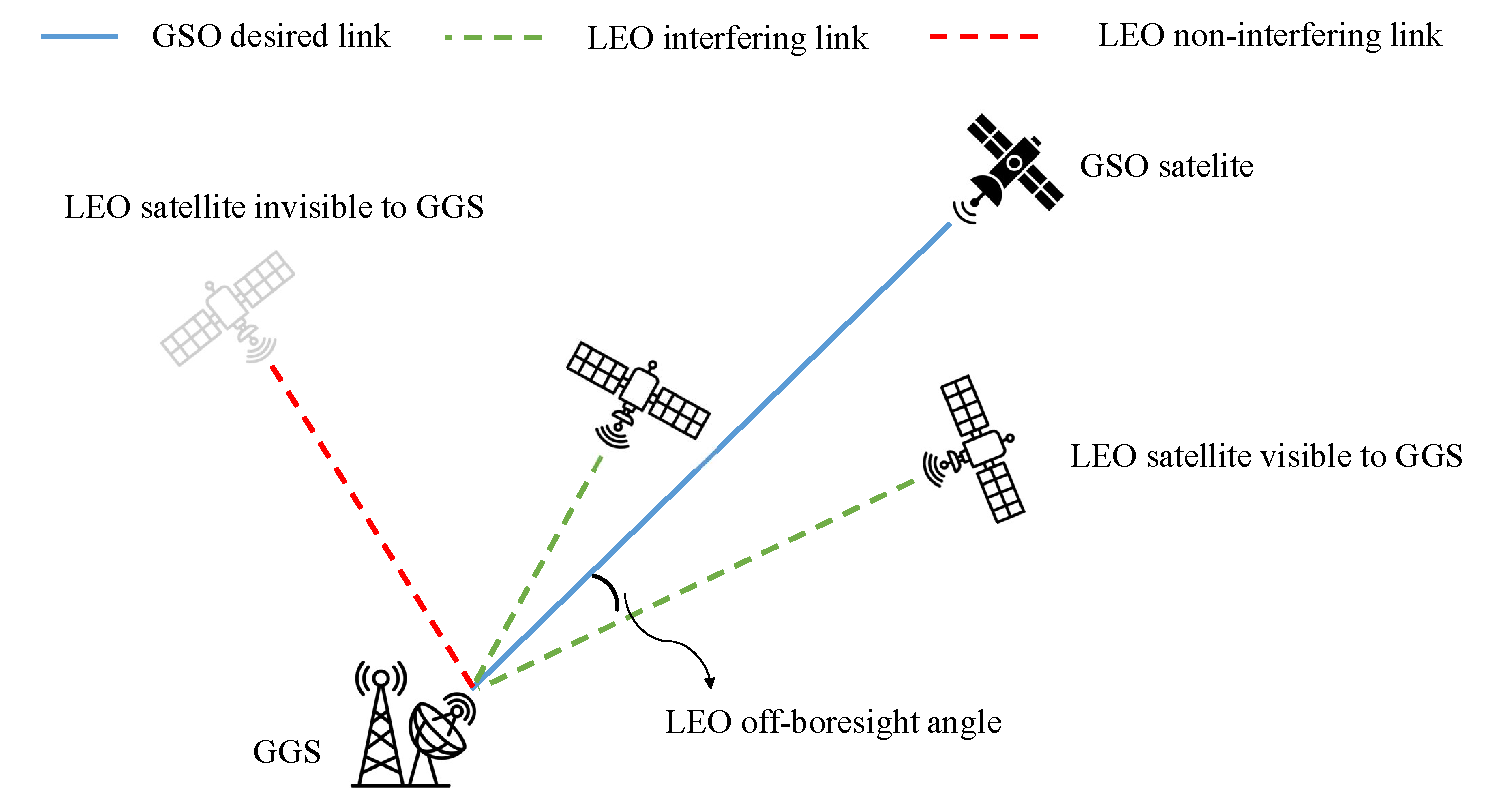
\includegraphics[width=\linewidth]{system-model.pdf}
    \caption{Interference scenario between GSO and LEO satellite systems.}
    \label{fig:interference-scenario}
\end{figure}

The received GSO carrier power is determined through classical satellite link relationships:
\begin{equation}
    C = \frac{\text{EIRP}_{\text{gso}} \cdot G_{\text{r, gso}}(\theta_0)}{L_{\text{FS, gso}} \cdot L_{\text{add}}}
    \label{eq:carrier_power}
\end{equation}
where $\text{EIRP}$ is GSO satellite equivalent isotropic radiated power, $G_{\text{r, gso}}(\theta_0)$ denotes the maximum receive antenna gain at boresight angle $\theta_0$, $L_{\text{FS, gso}}$ represents free-space path loss, and $L_{\text{add}}$ accounts for aggregate atmospheric impairments.

Interference contributions from $K$ LEO satellites are modeled as individual components:
\begin{equation}
    I_k = \frac{\text{EIRP}_k \cdot G_{\text{r, k}}(\theta_k) \cdot B_{\text{adj, k}}}{L_{\text{FS, k}} \cdot L_{\text{add}}}
    \label{eq:interference_power}
\end{equation}

The angular gain term $G_{\text{r, k}}(\theta_k)$ reflects spatial relationships caused by LEO orbital motion, while $B_{\text{adj, k}} \in [0,1]$ is the spectral overlap between GSO and LEO transmissions.

The signal received by physical layer at the GGS has three components:
\begin{align}
    y(t) =\, & x(t)\sqrt{\text{CNR}}\, (\text{Desired GSO}) \nonumber                                                 \\[0.5em]
             & + \sum_{k=1}^{K} i_k(t)e^{j2\pi \Delta f_k t}\sqrt{\text{INR}_k}\, (\text{LEO interference}) \nonumber \\[0.5em]
             & + \zeta(t)\, (\text{Thermal noise})
\end{align}
where $\Delta f_k = f_{\text{c},k} - f_{\text{c,gso}}$ captures carrier frequency offsets from Doppler effects. The exponential terms induce time-varying phase rotations proportional to relative satellite motion. Here, $\text{CNR}$ (Carrier-to-Noise Ratio) and $\text{INR}_k$ (Interference-to-Noise Ratio) respectively characterize the desired signal quality and interference intensity relative to the noise floor,

Dual signal representations are derived for machine learning processing:
\begin{itemize}
    \item Time-domain: $y^A$ captures instantaneous amplitude variations through uniform sampling
    \item Frequency-domain: Welch's power spectral density estimation generates logarithmic magnitude spectra via overlapping windowed transforms: $y^F = 10\log_{10}(\phi(y(t)))$
\end{itemize}

\subsection{Deep Learning Approaches for Interference Detection}
\label{ssec:related_works}

Recent advancements in machine learning have reshaped interference detection paradigms through a transition from traditional signal processing to anomaly discrimination. A popular strategy employs encoder-decoder architectures by training models to reconstruct idealized interference-free waveforms from raw inputs. This approach builds on the fundamental principle that interference anomalies create deviations from primary signals. Unlike regression-based methods that face challenges in modeling heterogeneous interference sources, reconstruction frameworks directly isolate deviations through input/output pattern comparisons.

Early implementations by Pellaco et al. \cite{pellacoSpectrumPredictionInterference2019} developed a long short-term memory autoencoder (LSTMAE) for detecting multi-scale anomalies in non-geostationary satellite signals, but its recursive architecture limits computational parallelism, leading to inference delays incompatible with latency-sensitive operations. Subsequent work by Saifaldawla et al. \cite{saifaldawlaConvolutionalAutoencodersNonGeostationary2024} addressed temporal dependency constraints through convolutional autoencoders (CAE), enabling direct in-phase/quadrature (IQ) sample processing for terrestrial interference detection.

Recent studies \cite{saifaldawlaGenAIBasedModelsNGSO2024} integrate transformer architectures into detection pipelines to resolve long-range spectral dependencies. Through self-attention mechanisms, these models achieve superior performance in capturing global interference signatures that conventional convolutional filters or recurrent units lack. Further innovations introduced dual-domain analysis by expanding input representations to joint time-frequency spaces.

Specifically, each input sample consisting of 800 sequential time-domain sampling points is first encoded through stacked transformer layers into a 128-dimensional latent representation. The decoder then inversely maps this latent space back to a reconstructed signal through learned upsampling operations. During training, a naïve mean squared error (MSE) loss between the original and reconstructed sequences drives the model to emulate interference-free waveform patterns. At inference, anomalous samples that deviate from interference-free signals will have a larger difference when reconstructed. Comparing this error with a predefined threshold will determine the presence of interference.

However, transformer-based detectors exhibit quadratic computational complexity growth with sequence length, posing challenges for wideband satellite implementations. Current approaches yet often employ seperated processing for temporal and spectral inputs, neglecting cross-domain correlations that could improve detection robustness through synergistic feature learning.

\section{Proposed Deep Learning Model}
\label{sec:model}

We propose DualAttWaveNet, an autoencoder that takes both time and frequency domain signal as input, and try to reconstruct both of them. The model consists of separate encoder and decoder for both domains, and a fusion module that utilizes bidirectional attention before concatenating. The loss function is regularized with wavelet transform to enforce reconstruction fidelity across multiple scales. The input signals from both time and frequency domain are of shape $B \times 800$, where $B$ is the batch size. After going through seperate convolution modules acting as downsampling layers, the signals are transformed into $B \times 128$ latent representations. Then these latent representations go through the bidirectional attention module and are concatenated before going through the upsampling layers. The final output is of shape $B \times 1600$. The model is trained with a combination of MSE loss and wavelet loss, described in Section \ref{subsec:wavelet}.

\subsection{Bidirectional Attention}
\label{subsec:bi_attn}

We propose a parameter-efficient mutual attention mechanism for cross-modal feature fusion. Unlike conventional multi-head attention in \cite{vaswaniAttentionAllYou2017}, our design employs single-head dot-product attention with spatial reduction to minimize computational overhead while maintaining inter-domain alignment capacity, as show in  \figurename~\ref{fig:bidirectional-attention}.

\begin{figure}[tb]
    \centering
    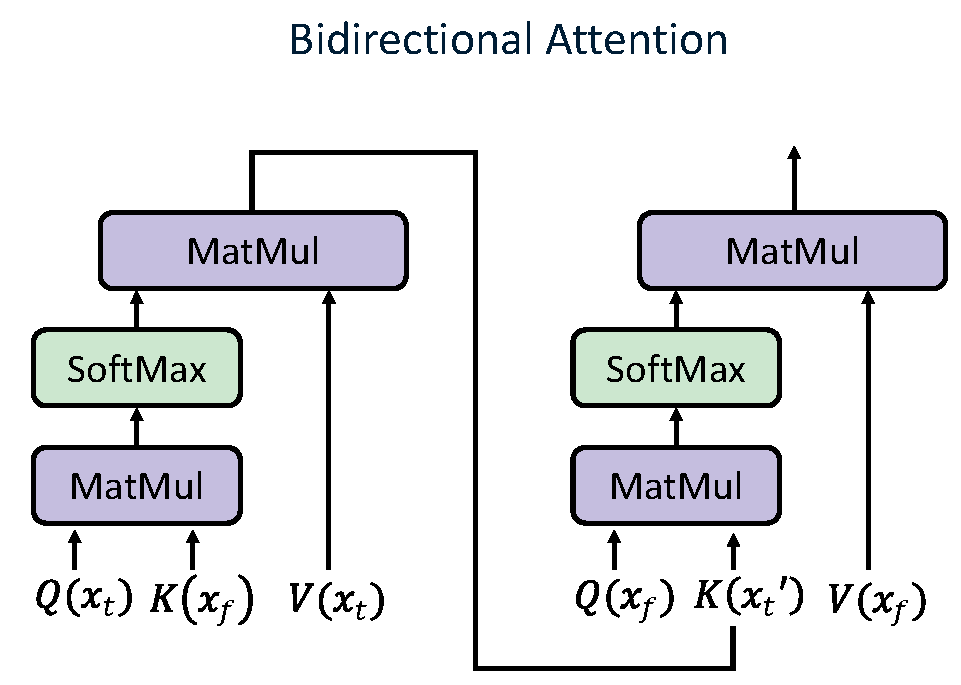
\includegraphics[width=0.9\linewidth]{bidirectional-attention.pdf}
    \caption{DualAttnWaveNet's bidirectional attention mechanism. Both attention phase share the same parameter $Q, K$ and $V$. To decrease channel numbers, they are implemented as 1d-Convolution.}
    \label{fig:bidirectional-attention}
\end{figure}

Given input feature maps $\mathbf{X} \in \mathbb{R}^{B \times C \times L}$ (temporal domain) and $\mathbf{Y} \in \mathbb{R}^{B \times C \times L}$ (spectral domain), the mutual attention operator computes:

\begin{equation}
    \begin{aligned}
        \text{MutualAttn}(\mathbf{X}, \mathbf{Y})    & = \mathbf{X} + \gamma \cdot \text{AttentionGate}(\mathbf{X}, \mathbf{Y})                        \\
        \text{AttentionGate}(\mathbf{X}, \mathbf{Y}) & = \mathbf{V}_y \cdot \text{Softmax}\left(\frac{\mathbf{Q}_x \mathbf{K}_y^\top}{\sqrt{d}}\right)
    \end{aligned}
\end{equation}

where $\gamma$ is a learnable scalar initialized to 0, $\mathbf{Q}_x = \mathcal{W}_Q(\mathbf{X}) \in \mathbb{R}^{B \times L \times \frac{C}{8}}$, $\mathbf{K}_y = \mathcal{W}_K(\mathbf{Y}) \in \mathbb{R}^{B \times \frac{C}{8} \times L}$, and $\mathbf{V}_y = \mathcal{W}_V(\mathbf{Y}) \in \mathbb{R}^{B \times C \times L}$. The projection matrices $\mathcal{W}_{Q,K,V}$ implement 1D convolutions with kernel size 1, reducing channel dimensions by $8\times$ for queries/keys to optimize memory footprint.

The compatibility scores between temporal ($\mathbf{X}$) and spectral ($\mathbf{Y}$) features are computed through matrix multiplication of the reduced-channel representations. This produces an $L \times L$ affinity matrix that represents position-wise cross-domain correlations before applying row-wise softmax normalization.

To preserve original feature stability during early training, the residual connection is initially dampened ($\gamma=0$) and progressively strengthened through learning. The symmetric architecture applies identical attention operations in both temporal→spectral and spectral→temporal directions, in sequential form:

\begin{equation}
    \begin{aligned}
        \mathbf{\widehat{X}} & = \text{MutualAttn}(\mathbf{X}, \mathbf{Y}) \\
        \mathbf{\widehat{Y}} & = \text{MutualAttn}(\mathbf{Y}, \mathbf{X})
    \end{aligned}
\end{equation}

This bidirectional design shares parameters across both call of attention, enables joint refinement of both modalities without major comutational overhead.

% \subsection{Wavelet-Domain Spectral Regularization}
% \label{subsec:wavelet}

% Our temporal-spectral analysis employs parameterized Morlet wavelets with learned scale distributions. Given input sequence $x \in \mathbb{R}^{B \times C \times L}$, we construct a filter bank $\mathcal{F} \in \mathbb{R}^{S \times 1 \times K}$ through:

% \begin{equation}
%     \mathcal{W}_s(\tau) = \operatorname{Norm} \left(\cos(\frac{1.75\tau}{2}) \odot \mathcal{G}(\tau,s)\right)
% \end{equation}

% where $\mathcal{G}(\tau,s) = \exp(-\tau^2/(2s^2))$ is the Gaussian window, $s \in \mathbb{S}$ denotes wavelet scales, and $K=4s_{\text{max}}$ defines the kernel size from maximum scale $s_{\text{max}}$. Each filter is $L_2$-normalized to preserve energy consistency across scales.

% The discrete wavelet transform is implemented as depth-wise separable convolution:

% \begin{equation}
%     \begin{aligned}
%         \mathbf{X}_{\text{wave}} & = \text{Conv1D}(\mathbf{X}, \mathcal{F})                                                                 \\
%                                  & = \bigcup_{s \in \mathbb{S}} \mathbf{X} \ast \mathcal{W}_s \in \mathbb{R}^{B \times C \times S \times L}
%     \end{aligned}
% \end{equation}

% where $\ast$ denotes cross-correlation with reflection padding for boundary alignment. The transform preserves temporal resolution through same-stride ($\text{stride}=1$) convolution across $S$ parallel scale dimensions. See \figurename~\ref{fig:wavelet-transform} for an illustration of the wavelet kernels and their input-output relationships.


% \begin{figure}[tb]
%     \centering
%     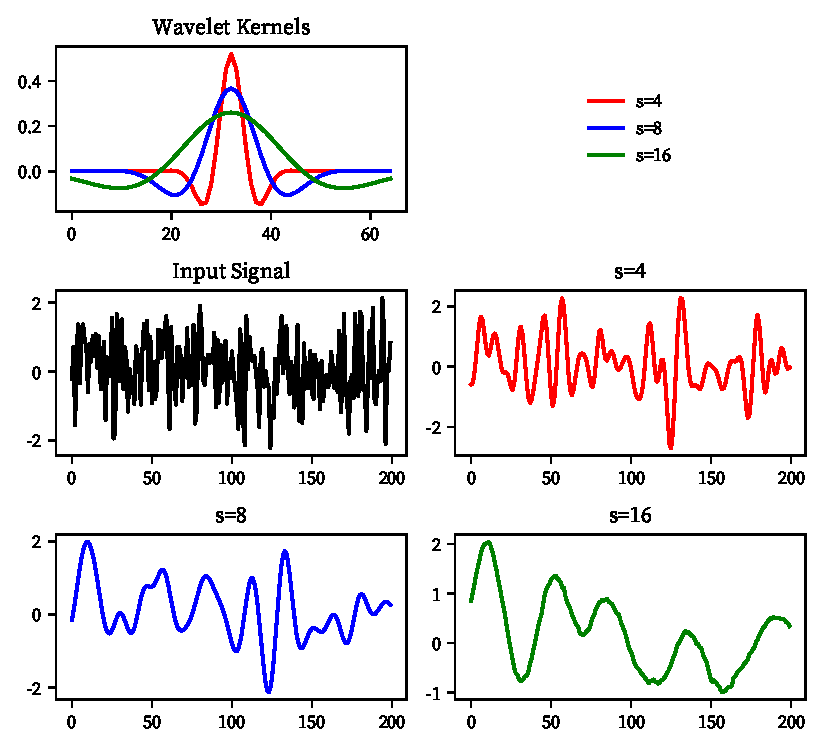
\includegraphics[width=\linewidth]{wavelet-transform.pdf}
%     \caption{(Top) Normalized Morlet-style wavelet kernels at scales [4, 8, 16]. (Bottom) Input–output relationships: Gaussian white noise input (top–left) and its filtered components using the respective wavelets (red: $s=4$, blue: $s=8$, green: $s=16$). Responses exhibit progressive high–frequency suppression and temporal smoothing with increasing scale. The visualizer implements bank normalization and preserves temporal resolution via same–padding convolutions (using a $\beta$–spline differentiable implementation).}

%     \label{fig:wavelet-transform}
% \end{figure}

% We optimize both signal-space and wavelet-domain reconstructions through:

% \begin{equation}
%     \mathcal{L} = \lambda_1 \|\mathbf{\hat{X}} - \mathbf{X}\|_2^2 + \lambda_2 \|\mathbf{\hat{X}}_{\text{wave}} - \mathbf{X}_{\text{wave}}\|_2^2
% \end{equation}

% where $\lambda_1=1$, $\lambda_2=0.5$ balance reconstruction error and wavelet transform loss.

\subsection{Wavelet-Domain Spectral Regularization}
\label{subsec:wavelet}

Traditional MSE loss  is not enough to capture the complex structure of the signal. We propose a wavelet loss term to enforce the reconstructed output to be consistent across all scales. Given an input tensor sequence $\mathbf{x} \in \mathbb{R}^{B \times C \times L}$ where $B$, $C$, and $L$ denote batch size, channels, and temporal length respectively, we construct a learnable filter bank $\mathcal{F} \in \mathbb{R}^{S \times 1 \times K}$ through the following parameterization:

\begin{equation}
    \label{eq:wavelet}
    \mathcal{W}_s(\tau) = \operatorname{Norm} \left(\cos\left(\frac{t}{s}\tau\right) \odot \mathcal{G}(\tau,s)\right)
\end{equation}

where $\mathcal{G}(\tau,s) = \exp(-\tau^2/(2s^2))$ represents the Gaussian envelope function, $s \in \mathbb{S}$ enumerates the wavelet scale parameters, and $K=4s_{\text{max}}$ determines the kernel size from the maximum scale $s_{\text{max}}$ to ensure sufficient spatial support. Each filter undergoes $L_2$-normalization to preserve energy consistency across multiple scales.

The discrete wavelet transform is implemented as asymmetric depth-wise separable convolution with spectral preservation properties:

\begin{equation}
    \begin{aligned}
        \mathbf{X}_{\text{wave}} & = \text{Conv1D}(\mathbf{X}, \mathcal{F})                                                                 \\
                                 & = \bigcup_{s \in \mathbb{S}} \mathbf{X} \ast \mathcal{W}_s \in \mathbb{R}^{B \times C \times S \times L}
    \end{aligned}
\end{equation}

Reflection padding strategy mitigates boundary artifacts while maintaining temporal resolution through stride-1 convolution across $S$ parallel scale dimensions. \figurename~\ref{fig:wavelet-transform} illustrates how wavelet kernels at different scales filter input signals.

\begin{figure}[tb]
    \centering
    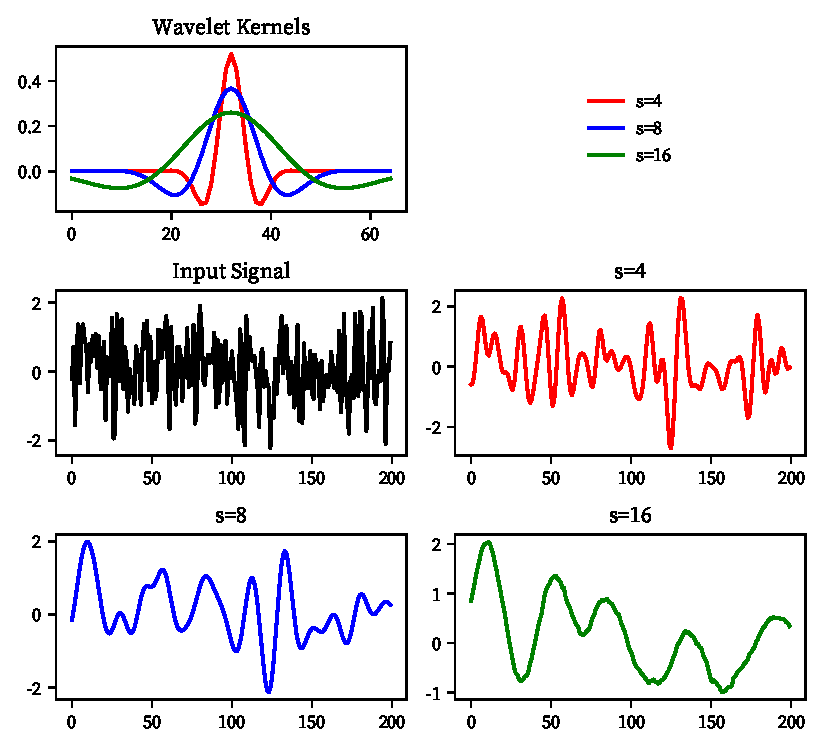
\includegraphics[width=\linewidth]{wavelet-transform.pdf}
    \caption{(Top) Normalized Morlet-style wavelet kernels at scales [4, 8, 16]. (Bottom) Input–output relationships: Gaussian white noise input (top–left) and its filtered components using the respective wavelets (red: $s=4$, blue: $s=8$, green: $s=16$). Responses exhibit progressive high–frequency suppression and temporal smoothing with increasing scale. The visualizer implements bank normalization and preserves temporal resolution via same–padding convolutions (using a $\beta$–spline differentiable implementation).}

    \label{fig:wavelet-transform}
\end{figure}

Our joint optimization framework combines both signal-space and wavelet-domain consistency through an adaptive loss weighting mechanism:

\begin{equation}
    \mathcal{L} = \lambda_1\|\mathbf{\hat{X}} - \mathbf{X}\|_{2}^2 + \lambda_2\sum_{s\in\mathbb{S}} \|\mathbf{\hat{X}}_{\text{wave}}^{(s)} - \mathbf{X}_{\text{wave}}^{(s)}\|_{2}^2
\end{equation}

where $\lambda_1$ and $\lambda_2$ represent empirically optimized weighting and the second term denotes the norm over wavelet subbands. This dual-domain regularization ensures simultaneous preservation of  temporal features and spectral distribution.

\subsection{Threshold Selection}

The final output of the model is a reconstructed signal. To determine whether the input signal contains interference, we compare the reconstructed signal with the original signal. If the difference is larger than a predefined threshold, we classify the input signal as interference. The threshold is determined by the following formula:

\begin{equation}
    \Gamma_{\text{th}} = \mu + \text{std}(\mathbf{L})
\end{equation}
where $\mu$ is the mean of the loss in validation set.  $\text{std}(\mathbf{L})$ is the standard deviation of the loss. This strategy assumes that the loss of the model on the validation set is normally distributed, and the threshold is set to be one standard deviation above the mean. Any loss above this threshold is considered outliers, hence containing interference.



\section{Experiments}
\label{sec:experiments}

\subsection{Data Configuration}

The synthetic dataset is generated through a 48-hour MATLAB simulation sampling Ku-band (10.7-12.7 GHz) interference scenarios at 10-second intervals, producing 17,281 temporal snapshots following \cite{saifaldawlaGenAIBasedModelsNGSO2024}. Each instance contains synchronized time-domain and frequency-domain representations: an 800-point waveform captures signal amplitudes, while an 800-bin spectral magnitude is derived via FFT processing.

Binary classification labels are assigned through link budget analysis, where class 0 denotes non-interference scenarios ($\text{INR} < \Gamma_{\text{th}}$) below the system protection threshold, and class 1 indicates substantial interference ($\text{INR} \geq \Gamma_{\text{th}}$) exceeding operational limits. We normalize the input signals in both domains separately to zero mean and unit variance.

The dataset is partitioned under anomaly detection constraints, with training (11,509 samples) and validation (1,302 samples) sets containing exclusively non-interference data (class 0). The test set comprises balanced proportions of 2,235 class 0 and 2,235 class 1 instances. The simulation incorporates time-varying link losses with 0-9 dB range, extreme interference cases reaching peak aggregate INR of 32.47 dB, with background CNR fluctuations between 6.40-15.40 dB.

\subsection{Baseline Models}

We use the following models as baselines to benchmark our framework: \textbf{LinearA}E with fully-connected encoder-decoder architectures as a simplistic reconstruction baseline; \textbf{CNNAE} utilizing 1D convolutional layers for encoder and MLP for decoder; \textbf{CNNAE+Attention} augmenting CNNAE with temporal self-attention modules; domain-specific \textbf{TrID} embedding spectral correlation priors; and \textbf{Transformer AE} constructed with stacked multi-head attention layers for global context modeling. All baselines adhere to the standard autoencoder paradigm that reconstructs inputs from bottleneck embeddings, implemented with identical training protocols and hyperparameter tuning strategies for fair comparison.

\subsection{Evaluation Results}

As shown in Table \ref{tab:main_results}, DualAttnWaveNet establishes state-of-the-art performance across all key metrics, showcasing its superior design synergy. It achieves the highest AUC score (0.9327), surpassing the best baseline (LinearAE/CNNAE: 0.9176) by 1.6\% and demonstrating a 36.9\% absolute improvement over the cumbersome Transformer AE (0.6812). Simultaneously, our framework completes inference in 0.5409s – 46\% of TrID's 1.0156s – while maintaining competitive F1 score parity (0.8351) with comparably lightweight models like CNNAE (0.8169). Notably, the F1 score shows only 0.3\% performance decay from the task-specialized TrID (0.8321), effectively balancing precision-recall tradeoffs through integrated dual-attention mechanisms.

\begin{table}[t]
    \caption{Performance Comparison of DualAttnWaveNet Against Baseline Models}
    \label{tab:main_results}
    \centering
    \resizebox{\linewidth}{!}{
        \begin{tabular}{lcccc}
            \toprule
            \textbf{Model}  & \textbf{Accuracy (\%) } $\uparrow$ & \textbf{F1 Score} $\uparrow$ & \textbf{AUC}$\uparrow$ & \textbf{Time(s)} $\downarrow$ \\
            \midrule
            DualAttnWaveNet & 0.8351                             & 0.8351                       & 0.9327                 & 0.5409                        \\
            \cmidrule{1-5}
            LinearAE        & 0.8149                             & 0.8149                       & 0.9176                 & 0.0966                        \\
            CNNAE           & 0.8170                             & 0.8169                       & 0.9175                 & 0.1654                        \\
            CNNAE+Attention & 0.7695                             & 0.7691                       & 0.8718                 & 0.5969                        \\
            TrID            & 0.8318                             & 0.8321                       & 0.8318                 & 1.0156                        \\
            Transformer AE  & 0.6812                             & 0.5921                       & 0.6812                 & 1.8354                        \\
            \bottomrule
        \end{tabular}}
\end{table}

Baseline analyses reveal critical architectural limitations: The Transformer AE's stacked multi-head attention layers incur huge latency (1.8354s) while suffering catastrophic performance collapse (-22.5\% F1 vs ours), exposing fundamental overparameterization issues. Although domain-specific TrID achieves near-parity accuracy (0.8318), its AUC score plunges to 0.8318 – diverging 10.8\% from our method – implying overfitting to spectral correlation priors. The temporal attention failure in CNNAE+Attention has computation time 3.6× over vanilla CNNAE (0.5969s vs 0.1654s) while degrading AUC by 5.2\%, contrasting sharply with our efficiently optimized dual-attention paradigm. LinearAE has the highest throughput (0.0966s) but suffers from suboptimal performance.

As visualized in \figurename~\ref{fig:roc_comparison}, the ROC curves quantify the discriminative power hierarchy among competing models. DualAttnWaveNet's left-skewed trajectory (AUC $=$ 0.9327) dominates the upper-left quadrant, achieving 83.5\% true positive rate at less than 10\% false positives. The performance collapse in ConvAE+Attention (AUC $=$ 0.8719) is shown as rightward curve drift, exposing the detrimental impact of ill-configured attention modules on feature selectivity. TransAE's trajectory (AUC $=$ 0.6812) hovers near the diagonal chance line, showing Transformer AE's failure to learn meaningful decision boundaries despite its 3.6× higher computational cost versus our method. \figurename~\ref{fig:confusion_matrix} reveals class-specific recognition patterns through confusion matrices across six models.

\begin{figure}[t]
    \centering
    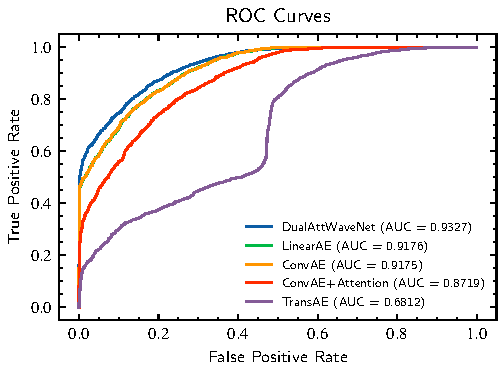
\includegraphics[width=\linewidth]{roc-comparison.pdf}
    \caption{ROC curves for DualAttnWaveNet and baseline models. DualAttnWaveNet achieves the highest AUC score.}
    \label{fig:roc_comparison}
\end{figure}

\begin{figure}[tb]
    \centering
    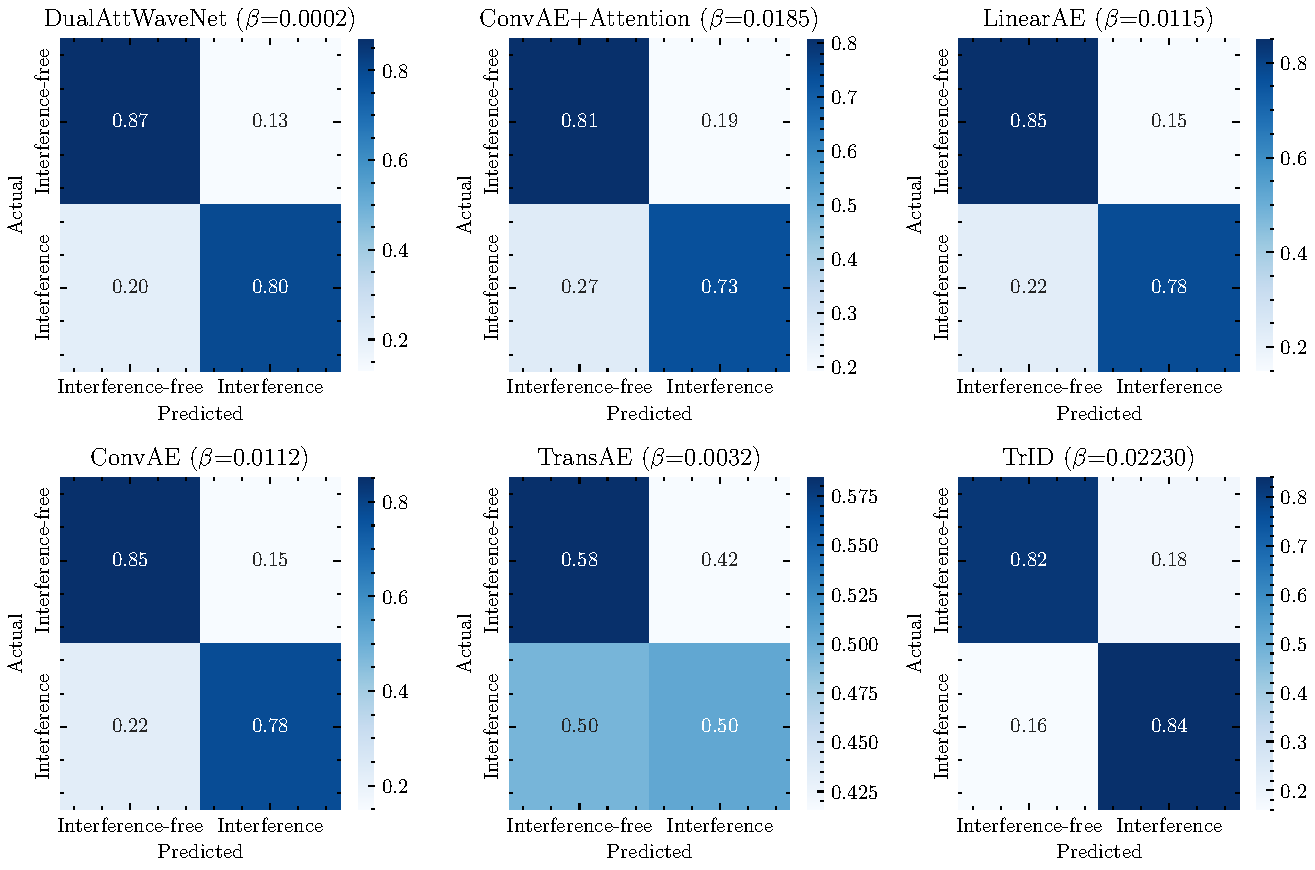
\includegraphics[width=\linewidth]{confusion.pdf}
    \caption{Confusion matrix for DualAttnWaveNet and baselines on the test set}
    \label{fig:confusion_matrix}
\end{figure}

The temporal localization parameter $t$ mentioned in Eq. \ref{eq:wavelet} governs the precision of interference feature extraction. The model achieves peak performance (0.9327 AUC) at t=2.  When $t=1$ introduces over-localization performance drops by 0.7\%. Conversely, larger t values gradually blur critical temporal details: $t=16$ cause 4.5\% AUC degradation. These findings confirm $t=2$ is the best choise for our model.

\begin{table}[tb]
    \centering
    \caption{Choosing Temporal Localization Parameter $t$}
    \label{tab:experiment-results}
    \begin{tabular}{cc}
        \toprule
        \textbf{t Value} & \textbf{Test AUC} \\
        \midrule
        1                & 0.9257            \\
        2                & \textbf{0.9327}   \\
        4                & 0.9221            \\
        8                & 0.9046            \\
        16               & 0.8874            \\
        \bottomrule
    \end{tabular}
\end{table}



\subsection{Ablation Study}

As shown in Table \ref{tab:ablation}, the full DualAttnWaveNet achieves the best performance with 83.51\% accuracy, 83.51\% F1 score, and 0.9327 AUC. Removing the mutual attention mechanism ("w/o Mutual Attention") causes consistent performance drops (0.6\% accuracy, 0.6\% F1, 0.3\% AUC). Disabling the wavelet loss ("w/o Wavelet Loss") further degrades accuracy by 1.0\%, proving the necessity of joint time-frequency optimization. The vanilla implementation exhibits significant performance limitations (79.95\% accuracy, 0.9175 AUC), demonstrating a 3.6\% accuracy gap compared to the full model, which highlights the collective contribution of our dual-attention design and spectral-aware constraints to robust classification capability.

\begin{table}[t]
    \caption{Ablation Study of DualAttnWaveNet Components}
    \label{tab:ablation}
    \centering

    \begin{tabular}{lccc}
        \toprule
        \textbf{Model Variant} & \textbf{Accuracy (\%)} $\uparrow$ & \textbf{F1 Score} $\uparrow$ & \textbf{AUC} $\uparrow$ \\
        \midrule
        DualAttnWaveNet (Full) & 0.8351                            & 0.8351                       & 0.9327                  \\
        \cmidrule{1-4}
        w/o Mutual Attention   & 0.8289                            & 0.8288                       & 0.9294                  \\
        w/o Wavelet Loss       & 0.8273                            & 0.8273                       & 0.9283                  \\
        Vanilla Implementation & 0.7995                            & 0.7975                       & 0.9175                  \\
        \bottomrule
    \end{tabular}

\end{table}

\section{Conclusion}
\label{sec:conclusion}

In this paper, we present DualAttWaveNet, a computationally-efficient multimodal framework for interference detection in GSO/LEO coexistence systems. We used a bidirectional attention mechanism to fuse time and frequency domain signals. This design integrates the capability of attention module and at the same time uses less computational resources. Additionally, we introduced a wavelet loss besides traditional MSE loss to enforce the reconstructed output to be consistent across all scales. Extensive evaluations in synthetic Ku-band scenarios show DualAttWaveNet achieves 0.9327 AUC with 83.51\% accuracy, surpassing state-of-the-art baselines TrID. The model is trained and tested on an edge NVIDIA 3050Ti GPU, demonstrating 50\% faster inference time compared to TrID while maintaining competitive F1 score. Future work will optimize spectral downsampling strategies for different spectrum overlaps scenarios.

\bibliographystyle{IEEEtran}
\bibliography{references}

\end{document}